\documentclass[final]{article}
\usepackage[paperwidth=48in,paperheight=36in,margin=0.30in]{geometry}
\usepackage{graphicx}
\usepackage[table]{xcolor}
\usepackage{booktabs}
\usepackage{array}
\usepackage{amsmath}
\usepackage{tikz}
\usepackage{hyperref}
\usepackage{lmodern}
\usepackage{microtype}
\usepackage{enumitem}
\renewcommand{\familydefault}{\sfdefault}

\pagestyle{empty}
\setlength{\parindent}{0pt}
\setlength{\parskip}{0.028in}
\setlength{\fboxsep}{0.09in}
\setlength{\fboxrule}{1.4pt}
\setlist[itemize]{leftmargin=0.24in,itemsep=0.012in,topsep=0.008in}

\definecolor{pagecream}{HTML}{F7F3E8}
\definecolor{panelwhite}{HTML}{FFFFFF}
\definecolor{templatedark}{HTML}{282622}
\definecolor{templateblue}{HTML}{0E2A55}
\definecolor{templateaccent}{HTML}{C36B4A}
\definecolor{tableblue}{HTML}{D7DEED}
\definecolor{tablebluealt}{HTML}{ECEFF7}
\definecolor{tablehead}{HTML}{38342E}
\definecolor{textblack}{HTML}{111111}

\pagecolor{templatedark}
\hypersetup{colorlinks=true,urlcolor=templateblue}

\newcounter{posterfigure}
\newcounter{postertable}

\newcommand{\bodytext}{\fontsize{18.0}{21.6}\selectfont}
\newcommand{\smalltext}{\fontsize{12.8}{15.3}\selectfont}
\newcommand{\captionfont}{\fontsize{11.8}{14.0}\selectfont}
\newcommand{\tabletext}{\fontsize{18.4}{21.2}\selectfont}
\newcommand{\tablecaptionfont}{\fontsize{15.6}{18.4}\selectfont}
\newcommand{\figuretext}{\fontsize{16.8}{20.0}\selectfont}
\newcommand{\subhead}[1]{{\fontsize{19.8}{23.4}\selectfont\bfseries\color{templateblue}#1}\par}
\newcommand{\paneltitle}[1]{{\fontsize{29.2}{33.4}\selectfont\bfseries\color{textblack}#1}\par\vspace{0.030in}}
\newcommand{\contentpanel}[2]{%
  \fcolorbox{templatedark}{panelwhite}{%
    \begin{minipage}[t][#1][t]{\dimexpr\linewidth-2\fboxsep-2\fboxrule\relax}
    #2
    \end{minipage}%
  }%
}
\newcommand{\figcaption}[1]{%
  \refstepcounter{posterfigure}%
  \par\begin{center}{\captionfont\color{textblack}\textbf{Figure \theposterfigure.} #1\par}\end{center}%
}
\newcommand{\tabcaption}[1]{%
  \refstepcounter{postertable}%
  {\tablecaptionfont\color{textblack}\textbf{Table \thepostertable.} #1\par}%
  \vspace{0.018in}%
}
\newcommand{\metric}[2]{%
  \begin{minipage}[t]{0.30\linewidth}
  \centering
  {\fontsize{35}{39}\selectfont\bfseries\color{templateaccent}#1}\par
  {\smalltext\color{textblack}#2}
  \end{minipage}
}

\begin{document}
\bodytext\color{textblack}

\noindent
\colorbox{pagecream}{%
  \begin{minipage}[t][1.75in][c]{0.602\linewidth}
  \resizebox{\linewidth}{!}{\bfseries Toward Substrate-Agnostic SERS Classification Using Siamese Metric Learning}
  \end{minipage}%
}%
\hfill
\colorbox{templatedark}{%
  \begin{minipage}[t][1.75in][c]{0.340\linewidth}
  \raggedleft\color{white}
  {\fontsize{25}{29}\selectfont\bfseries Jesse Levine$^{1,*}$, Hal Bowen-Smith$^{1}$, Greg Wardle$^{1}$, and Dr. Li-Lin Tay$^{1}$}\par
  \vspace{0.07in}
  {\fontsize{18}{21}\selectfont $^{1}$Metrology Research Centre, National Research Council Canada, Ottawa, ON, Canada}\par
  \vspace{0.06in}
  {\fontsize{15.5}{18}\selectfont $^{*}$Jesse.Levine@nrc-cnrc.gc.ca}
  \end{minipage}%
}

\vspace{0.14in}

\begin{minipage}[t]{0.49\linewidth}
\contentpanel{5.85in}{%
\paneltitle{BACKGROUND / MOTIVATION}
\subhead{SERS vs. standard Raman}
Standard Raman measures a molecule's vibrational fingerprint directly, but the scattering signal is weak. Surface-enhanced Raman spectroscopy (SERS) uses nanostructured metal substrates to amplify Raman scattering, enabling more sensitive detection. That gain comes with a complication: the measured spectrum can depend on the substrate, surface binding, and local enhancement hotspots, not only on the chemical identity.

\vspace{0.12in}
\subhead{Why substrate agnosticism matters}
A useful SERS classifier should report the \textbf{chemical analyte}, not the sensor condition it was measured on. If the model relies on substrate-specific fingerprints, strong accuracy can fail when the same chemical is measured on a different substrate, batch, or vendor format. The goal is therefore not only high accuracy, but a representation that preserves analyte identity while reducing substrate identity.

\vspace{0.14in}
\subhead{The shift in target}
\textbf{Stage 1} asked which measured chemical-substrate pair produced the spectrum, for example 4NP on Ag or benzenethiol on PICO. \textbf{Stage 2} asks which chemical produced the spectrum while an entire substrate family is withheld from training.

\vspace{0.14in}
\subhead{Central question}
Can a Siamese encoder learn a representation where spectra from the same chemical are close together even when the substrate changes?

\vspace{0.20in}
\begin{center}
\resizebox{0.66\linewidth}{!}{%
\begin{tikzpicture}[x=1in,y=1in,font=\figuretext]
\node[draw=templatedark,fill=pagecream,rounded corners=0.07in,minimum width=3.65in,minimum height=0.78in,align=center,line width=1.1pt] (s1) at (0,0) {\textbf{Substrates}\\PICO, pSERS\\printed Ag/Au paper};
\node[draw=templatedark,fill=pagecream,rounded corners=0.07in,minimum width=3.65in,minimum height=0.78in,align=center,line width=1.1pt] (s2) at (4.25,0) {\textbf{Analyte exposure}\\Soak in diluted analyte\\for 1 h};
\node[draw=templatedark,fill=pagecream,rounded corners=0.07in,minimum width=3.65in,minimum height=0.78in,align=center,line width=1.1pt] (s3) at (8.5,0) {\textbf{Dry}\\Before measurement};
\node[draw=templatedark,fill=pagecream,rounded corners=0.07in,minimum width=3.65in,minimum height=0.78in,align=center,line width=1.1pt] (s4) at (12.75,0) {\textbf{Raman spectrometer}\\Horiba LabRAM HR800\\Raw SERS spectrum};
\draw[->,line width=1.8pt,color=templateblue] (s1) -- (s2);
\draw[->,line width=1.8pt,color=templateblue] (s2) -- (s3);
\draw[->,line width=1.8pt,color=templateblue] (s3) -- (s4);
\end{tikzpicture}%
}
\end{center}
\figcaption{Sample-preparation workflow. Commercial PICO and pSERS sensors are used alongside in-house printed Ag/Au nanoparticle-paper substrates. Each analyte-substrate preparation is soaked, dried, and measured on a Horiba LabRAM HR800 Raman spectrometer as a raw spectrum before preprocessing.}
}
\end{minipage}
\hfill
\begin{minipage}[t]{0.49\linewidth}
\contentpanel{7.55in}{%
\paneltitle{SAMPLES}
\vspace{0.16in}
\subhead{How samples were prepared}
Two substrate types were measured: commercial PICO/pSERS sensors and in-house Ag/Au nanoparticle paper. The Ag/Au substrates were prepared by inkjet-printing colloidal nanoparticle solution onto filter paper. For each chemical-substrate condition, the substrate was soaked in a diluted analyte solution for 1 h, removed, allowed to dry, and then measured on a Horiba LabRAM HR800 Raman spectrometer as raw SERS intensity versus Raman shift.

\vspace{0.24in}
\subhead{Current chemical-by-substrate matrix}
After grouping AgNP with Ag and AuNP with Au, benzenethiol and pyridine span all four substrate families. 4NP is missing on Au because it does not respond there.

\vspace{0.30in}
\begin{center}
\begin{minipage}{0.55\linewidth}
\tabcaption{Measured chemical-by-substrate matrix after grouping AgNP with Ag and AuNP with Au. A dash marks a missing or unusable chemical-substrate condition.}
\centering
\tabletext
\begingroup
\setlength{\tabcolsep}{11pt}
\renewcommand{\arraystretch}{1.08}
\begin{tabular}{@{}lcccc@{}}
\toprule
\textbf{Chemical} & \textbf{Ag} & \textbf{Au} & \textbf{PICO} & \textbf{pSERS} \\
\midrule
4NP & yes & -- & yes & yes \\
Benzenethiol & yes & yes & yes & yes \\
Pyridine & yes & yes & yes & yes \\
DMF & -- & yes & -- & -- \\
\bottomrule
\end{tabular}
\endgroup
\end{minipage}
\end{center}

\vspace{0.24in}
\subhead{4NP on Au}
4NP is missing on Au for chemical reasons rather than only missing data: it has poor attraction to the gold substrate and does not produce a usable SERS response under these sample conditions.

\vspace{0.20in}
\subhead{Dataset implication}
The matrix is structurally incomplete, so the result should be read as a controlled transfer study rather than a universal SERS classifier. Broader chemical coverage across every substrate family is still needed before claiming general substrate-agnostic detection.
}
\end{minipage}

\vspace{0.09in}

\begin{minipage}[t]{0.49\linewidth}
\vspace{-1.70in}
\contentpanel{22.10in}{%
\paneltitle{CHEMICAL-SUBSTRATE CLASSIFICATION}
\subhead{What the first model solved}
The first successful Siamese model predicted \textbf{pair labels}. This established that the spectra contain reproducible chemical-surface signatures and that a shared Conv1D encoder can compare spectra by nearest reference in embedding space. It was a useful baseline, but the substrate remained part of the class.

\vspace{0.18in}
{\fontsize{24}{28}\selectfont\bfseries\color{templateaccent}98.76\%}\hspace{0.08in}{\bodytext top-1 pair-classification accuracy on 403 query spectra.}\par

\vspace{0.40in}
\begin{center}
\begin{minipage}[t]{0.86\linewidth}
\centering
\resizebox{1.00\linewidth}{!}{%
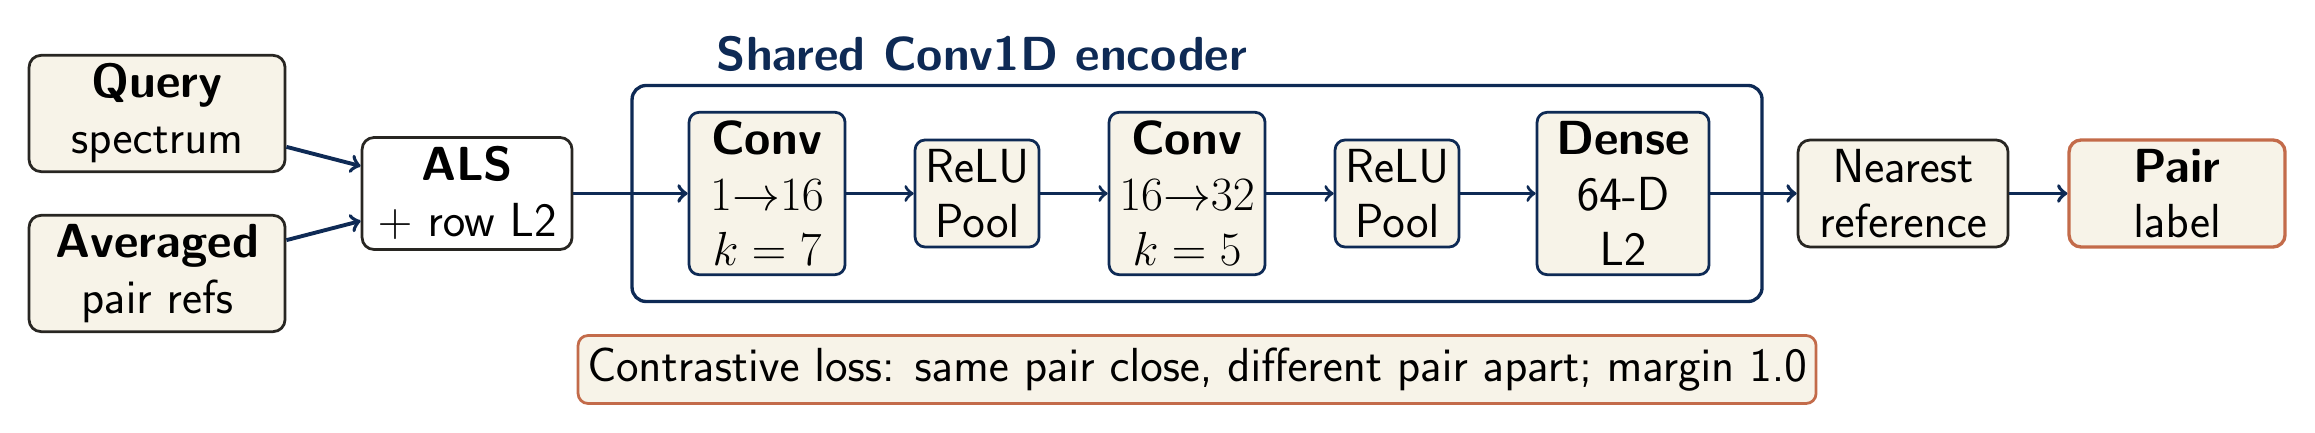
\begin{tikzpicture}[x=1in,y=1in,font=\figuretext]
\node[draw=templatedark,fill=pagecream,rounded corners=0.06in,minimum width=1.28in,minimum height=0.48in,align=center,line width=1pt] (q) at (0,1.38) {\textbf{Query}\\spectrum};
\node[draw=templatedark,fill=pagecream,rounded corners=0.06in,minimum width=1.28in,minimum height=0.48in,align=center,line width=1pt] (r) at (0,0.58) {\textbf{Averaged}\\pair refs};
\node[draw=templatedark,fill=panelwhite,rounded corners=0.06in,minimum width=1.05in,minimum height=0.56in,align=center,line width=1pt] (pre) at (1.55,0.98) {\textbf{ALS}\\+ row L2};

\node[draw=templateblue,fill=panelwhite,rounded corners=0.07in,minimum width=5.65in,minimum height=1.08in,line width=1.2pt] (encbox) at (5.20,0.98) {};
\node[anchor=west,color=templateblue] at (2.75,1.68) {\textbf{Shared Conv1D encoder}};
\node[draw=templateblue,fill=pagecream,rounded corners=0.05in,minimum width=0.78in,minimum height=0.54in,align=center,line width=1pt] (c1) at (3.05,0.98) {\textbf{Conv}\\$1{\to}16$\\$k=7$};
\node[draw=templateblue,fill=pagecream,rounded corners=0.05in,minimum width=0.62in,minimum height=0.48in,align=center,line width=1pt] (p1) at (4.10,0.98) {ReLU\\Pool};
\node[draw=templateblue,fill=pagecream,rounded corners=0.05in,minimum width=0.78in,minimum height=0.54in,align=center,line width=1pt] (c2) at (5.15,0.98) {\textbf{Conv}\\$16{\to}32$\\$k=5$};
\node[draw=templateblue,fill=pagecream,rounded corners=0.05in,minimum width=0.62in,minimum height=0.48in,align=center,line width=1pt] (p2) at (6.20,0.98) {ReLU\\Pool};
\node[draw=templateblue,fill=pagecream,rounded corners=0.05in,minimum width=0.86in,minimum height=0.54in,align=center,line width=1pt] (emb) at (7.33,0.98) {\textbf{Dense}\\64-D\\L2};

\node[draw=templatedark,fill=pagecream,rounded corners=0.06in,minimum width=1.05in,minimum height=0.48in,align=center,line width=1pt] (d) at (8.73,0.98) {Nearest\\reference};
\node[draw=templateaccent,fill=pagecream,rounded corners=0.06in,minimum width=1.08in,minimum height=0.48in,align=center,line width=1.2pt] (out) at (10.10,0.98) {\textbf{Pair}\\label};

\node[draw=templateaccent,fill=pagecream,rounded corners=0.05in,minimum width=5.65in,minimum height=0.34in,align=center,line width=1pt] at (5.20,0.10) {Contrastive loss: same pair close, different pair apart; margin 1.0};

\draw[->,line width=1.4pt,color=templateblue] (q) -- (pre);
\draw[->,line width=1.4pt,color=templateblue] (r) -- (pre);
\draw[->,line width=1.4pt,color=templateblue] (pre) -- (c1);
\draw[->,line width=1.2pt,color=templateblue] (c1) -- (p1);
\draw[->,line width=1.2pt,color=templateblue] (p1) -- (c2);
\draw[->,line width=1.2pt,color=templateblue] (c2) -- (p2);
\draw[->,line width=1.2pt,color=templateblue] (p2) -- (emb);
\draw[->,line width=1.4pt,color=templateblue] (emb) -- (d);
\draw[->,line width=1.4pt,color=templateblue] (d) -- (out);
\end{tikzpicture}%
}
\end{minipage}
\end{center}
\refstepcounter{posterfigure}
\par\begin{center}{\captionfont\color{textblack}\textbf{Figure \theposterfigure.} Stage 1 Siamese pair-classification architecture and inference. Query spectra and averaged pair references are baseline corrected, row-L2 normalized, and passed through the same two-block Conv1D encoder. The nearest 64-D reference embedding gives the chemical-substrate pair label.\par}\end{center}

\vspace{0.44in}
\noindent
\begin{minipage}[t]{0.52\linewidth}
\vspace{2.5in}
\begin{center}
\begin{minipage}{0.78\linewidth}
\tabcaption{Stage 1 data support. A stratified 20/80 split used 100 training spectra and 403 query spectra. Most pair classes contributed 5 train and 20 query spectra; DMF/Au contributed 45 train and 183 query spectra. Inference used one averaged reference per pair class.}
\centering
\tabletext
\begingroup
\setlength{\tabcolsep}{5pt}
\renewcommand{\arraystretch}{1.04}
\begin{tabular}{@{}lr@{}}
\toprule
\textbf{Quantity} & \textbf{Count} \\
\midrule
Pair classes & 12 \\
Total spectra & 503 \\
Training spectra & 100 \\
Query spectra & 403 \\
Averaged references & 12 \\
References per pair & 1 \\
Typical train/query per pair & 5 / 20 \\
DMF/Au train/query & 45 / 183 \\
\bottomrule
\end{tabular}
\endgroup
\end{minipage}
\end{center}
\end{minipage}
\hfill
\begin{minipage}[t]{0.39\linewidth}
\vspace{0.65in}
\centering
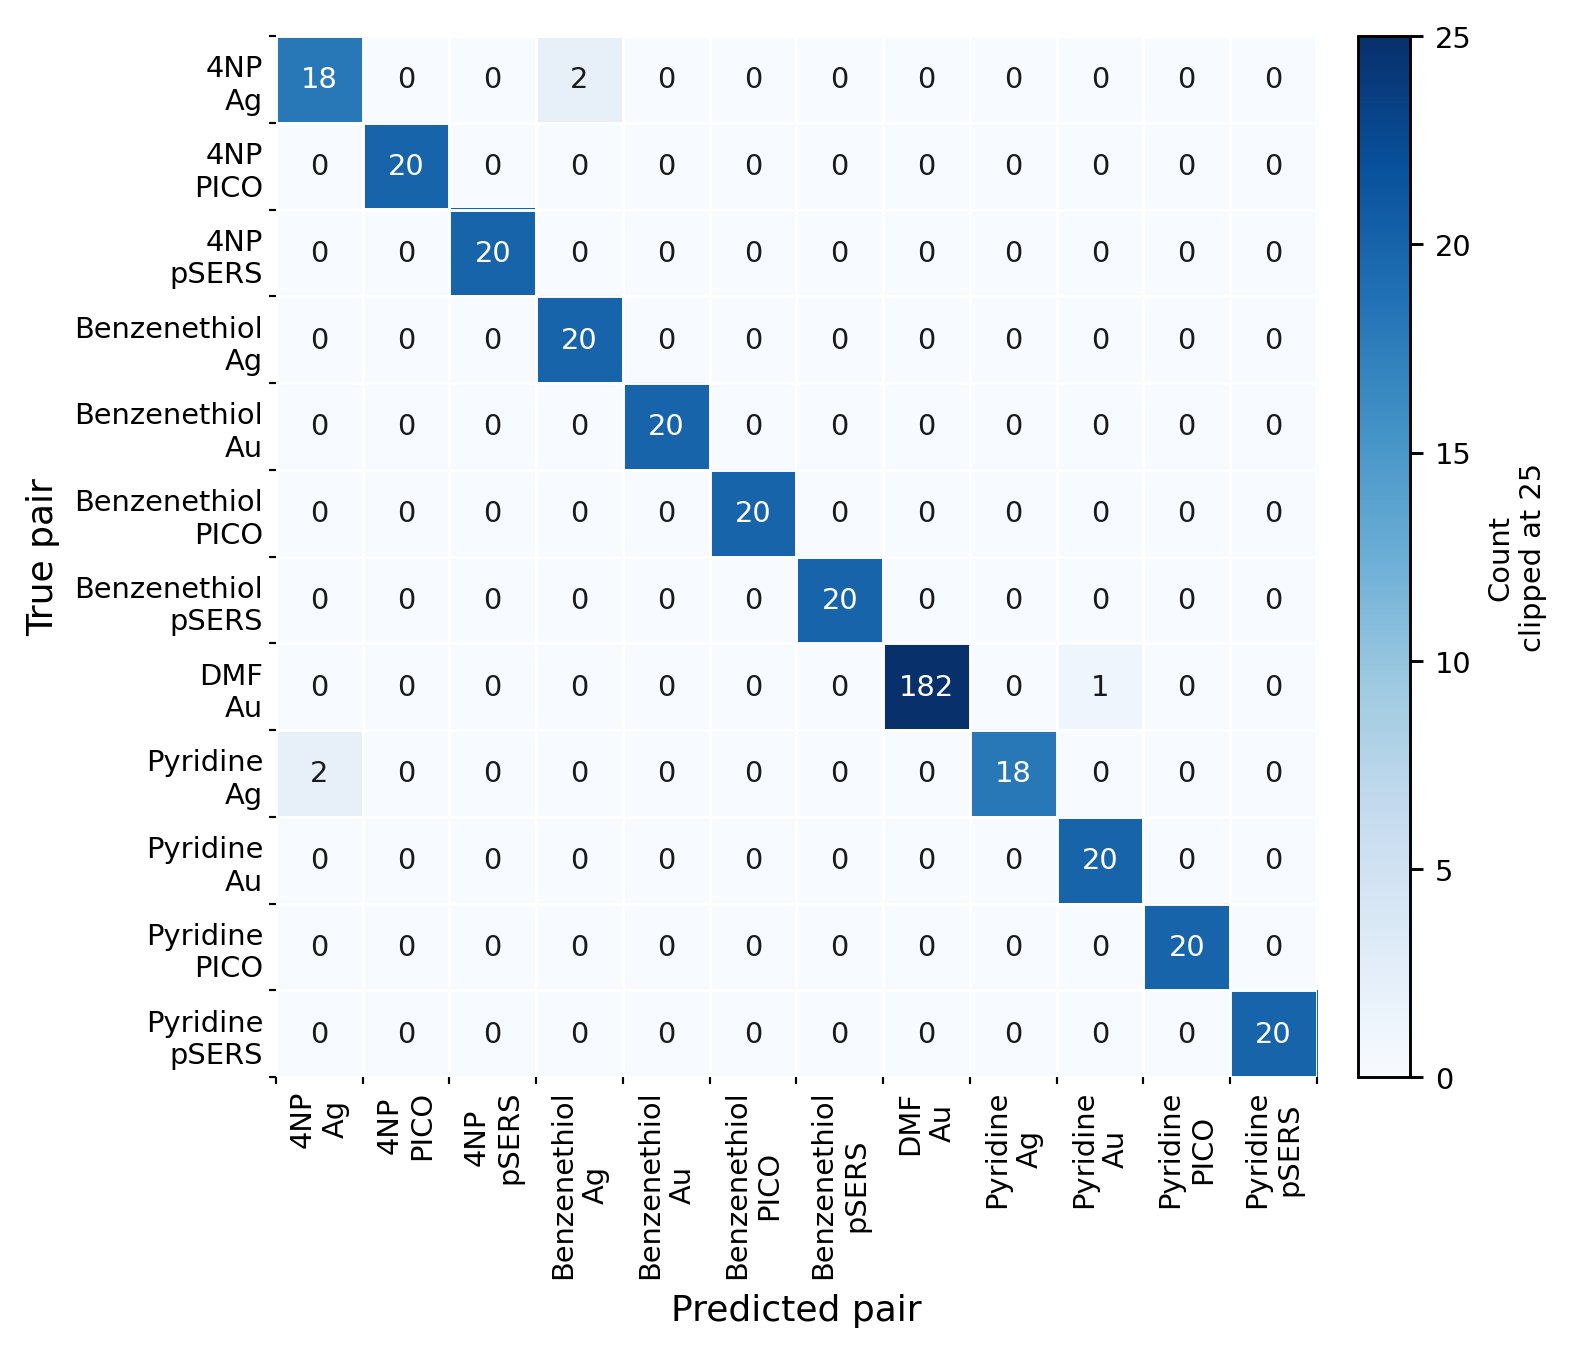
\includegraphics[width=1.00\linewidth]{figures/stage1_pair_confusion_matrix.png}
\figcaption{Stage 1 confusion matrix for chemical-substrate pair classification on 403 query spectra. Rows are true measured pairs and columns are predicted pairs; diagonal cells are correct assignments. The near-perfect diagonal gives 98.76\% top-1 accuracy, showing that the Siamese model reliably matches spectra to measured analyte-surface pairs. This is strong pair recognition, not substrate-agnostic chemical recognition, because the target label still combines the analyte and substrate.}
\end{minipage}

\vfill
\vspace{-3.45in}
\begin{center}
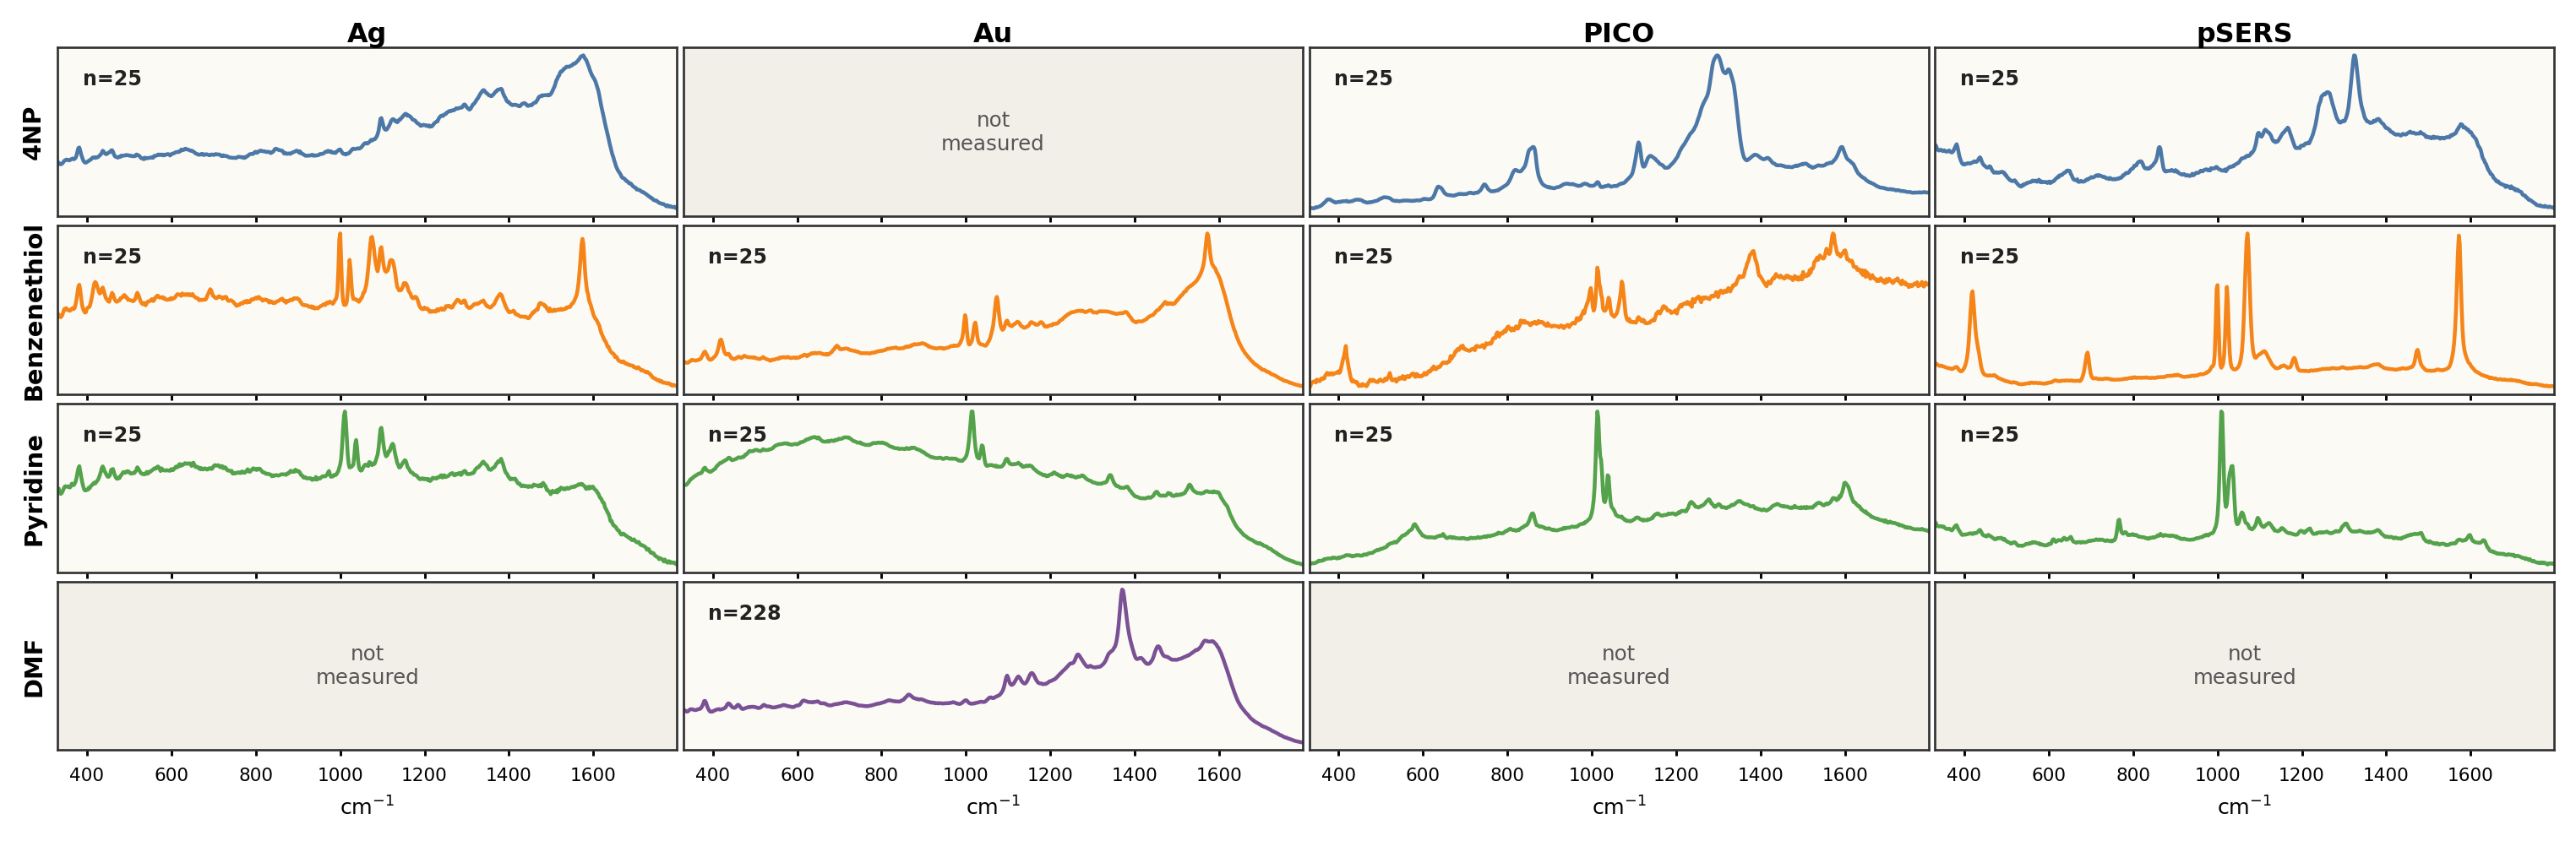
\includegraphics[width=0.66\linewidth]{figures/average_spectra_by_pair_compact.png}
\end{center}
\figcaption{Average raw SERS spectrum for each measured chemical-substrate family used to motivate Stage 1 pair classification. Each panel is cropped to 330--1800 cm$^{-1}$ and independently min-max scaled, so the comparison emphasizes peak positions and spectral shape rather than absolute intensity. The figure shows why the first task was easier than substrate-agnostic detection: the model could learn reproducible analyte-surface signatures, including substrate-dependent spectral structure.}
}

\vspace{0.24in}

\contentpanel{4.00in}{%
\paneltitle{TAKEAWAYS AND FUTURE DIRECTIONS}
\begin{minipage}[t]{0.43\linewidth}
\vspace{0pt}
\smalltext
\subhead{Takeaways}
\vspace{0.16in}
\begin{itemize}
\item Stage 1 proved the spectra are classifiable, but only as measured analyte-surface pairs.
\item Stage 2 keeps Siamese metric learning while making the target stricter: chemical identity on an unseen substrate family.
\item Triplet training improves chemical organization in embedding space and reduces substrate organization.
\item The main weakness is localized to 4NP on held-out Ag, where substrate chemistry may change the measured target.
\end{itemize}
\end{minipage}
\hfill
\begin{minipage}[t]{0.34\linewidth}
\vspace{0pt}
\smalltext
\subhead{Future directions}
\vspace{0.16in}
\begin{itemize}
\item Fill the chemical-by-substrate matrix with responsive analytes measured across Ag, Au, PICO, and pSERS.
\item Add independent preparations, measurement days, and map locations so transfer is tested across real experimental variation.
\item Prioritize Ag-family 4NP controls and reaction-product checks before treating the Ag error as model-only.
\end{itemize}
\end{minipage}
\hfill
\begin{minipage}[t]{0.17\linewidth}
\vspace{0pt}
\centering
{\fontsize{15}{18}\selectfont\bfseries\color{templateblue}ACKNOWLEDGMENTS}\par
\vspace{0.26in}

\includegraphics[width=0.90\linewidth]{figures/logos/nrc_logo.png}
\end{minipage}
}
\end{minipage}
\hfill
\begin{minipage}[t]{0.505\linewidth}
\contentpanel{24.98in}{%
\vspace{0.70in}
\paneltitle{SUBSTRATE-AGNOSTIC MODEL}
{\fontsize{24}{28}\selectfont\bfseries\color{templateaccent}97.5\%}\hspace{0.08in}{\bodytext mean fold accuracy across leave-one-substrate-family-out chemical-label tests. Each fold withholds one substrate family from training, so success requires chemical transfer to an unseen surface.}\par

\vspace{0.14in}
\subhead{Architecture and training}
\begin{center}
\begin{minipage}[t]{0.86\linewidth}
\centering
\resizebox{1.00\linewidth}{!}{%
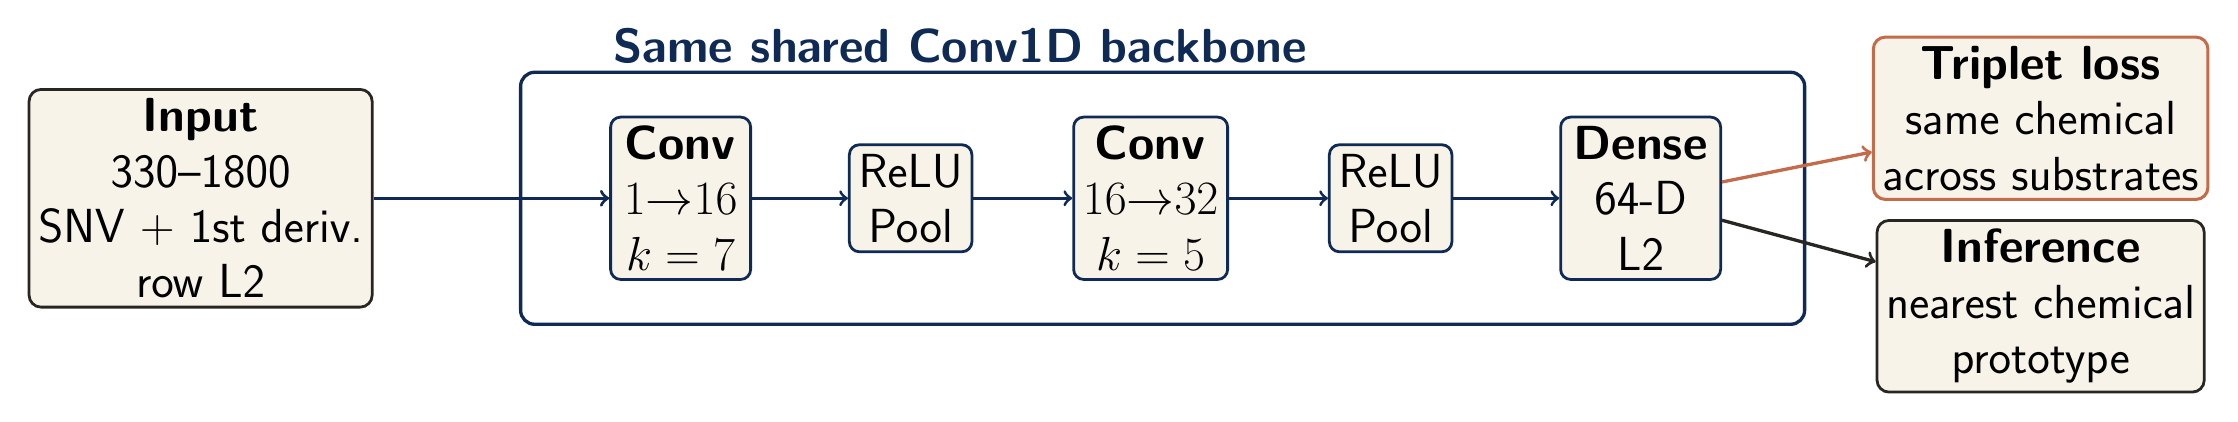
\begin{tikzpicture}[x=1in,y=1in,font=\figuretext]
\node[draw=templatedark,fill=pagecream,rounded corners=0.06in,minimum width=1.18in,minimum height=0.58in,align=center,line width=1pt] (input) at (-0.35,1.12) {\textbf{Input}\\330--1800\\SNV + 1st deriv.\\row L2};

\node[draw=templateblue,fill=panelwhite,rounded corners=0.07in,minimum width=6.42in,minimum height=1.26in,line width=1.2pt] (encbox) at (4.46,1.12) {};
\node[anchor=west,fill=panelwhite,text=templateblue,inner xsep=0.06in,inner ysep=0.01in] at (1.65,1.88) {\textbf{Same shared Conv1D backbone}};
\node[draw=templateblue,fill=pagecream,rounded corners=0.05in,minimum width=0.70in,minimum height=0.50in,align=center,line width=1pt] (c1) at (2.05,1.12) {\textbf{Conv}\\$1{\to}16$\\$k=7$};
\node[draw=templateblue,fill=pagecream,rounded corners=0.05in,minimum width=0.55in,minimum height=0.44in,align=center,line width=1pt] (p1) at (3.20,1.12) {ReLU\\Pool};
\node[draw=templateblue,fill=pagecream,rounded corners=0.05in,minimum width=0.70in,minimum height=0.50in,align=center,line width=1pt] (c2) at (4.40,1.12) {\textbf{Conv}\\$16{\to}32$\\$k=5$};
\node[draw=templateblue,fill=pagecream,rounded corners=0.05in,minimum width=0.55in,minimum height=0.44in,align=center,line width=1pt] (p2) at (5.60,1.12) {ReLU\\Pool};
\node[draw=templateblue,fill=pagecream,rounded corners=0.05in,minimum width=0.80in,minimum height=0.50in,align=center,line width=1pt] (emb) at (6.85,1.12) {\textbf{Dense}\\64-D\\L2};

\node[draw=templateaccent,fill=pagecream,rounded corners=0.06in,minimum width=1.55in,minimum height=0.58in,align=center,line width=1.1pt] (loss) at (8.85,1.52) {\textbf{Triplet loss}\\same chemical\\across substrates};
\node[draw=templatedark,fill=pagecream,rounded corners=0.06in,minimum width=1.55in,minimum height=0.58in,align=center,line width=1pt] (proto) at (8.85,0.58) {\textbf{Inference}\\nearest chemical\\prototype};

\draw[->,line width=1.2pt,color=templateblue] (input) -- (c1);
\draw[->,line width=1.1pt,color=templateblue] (c1) -- (p1);
\draw[->,line width=1.1pt,color=templateblue] (p1) -- (c2);
\draw[->,line width=1.1pt,color=templateblue] (c2) -- (p2);
\draw[->,line width=1.1pt,color=templateblue] (p2) -- (emb);
\draw[->,line width=1.2pt,color=templateaccent] (emb) -- (loss);
\draw[->,line width=1.2pt,color=templatedark] (emb) -- (proto);
\end{tikzpicture}%
}
\figcaption{Substrate-agnostic Siamese architecture and training. The encoder keeps the same two-block Conv1D backbone as the pair-classification model, but the target changes from chemical-substrate pair identity to chemical identity. Cropped, SNV-normalized first-derivative spectra are embedded with triplet loss, which pulls same-chemical spectra together across substrates before nearest-prototype chemical inference. Training used Adam with learning rate $10^{-3}$, batch size 32, 100 epochs, CUDA/GPU execution, and triplet margin 0.2.}
\end{minipage}
\end{center}

\vspace{0.35in}
\noindent
\begin{minipage}[t]{0.46\linewidth}
\vspace{0.52in}
\centering
\scalebox{1}[1.10]{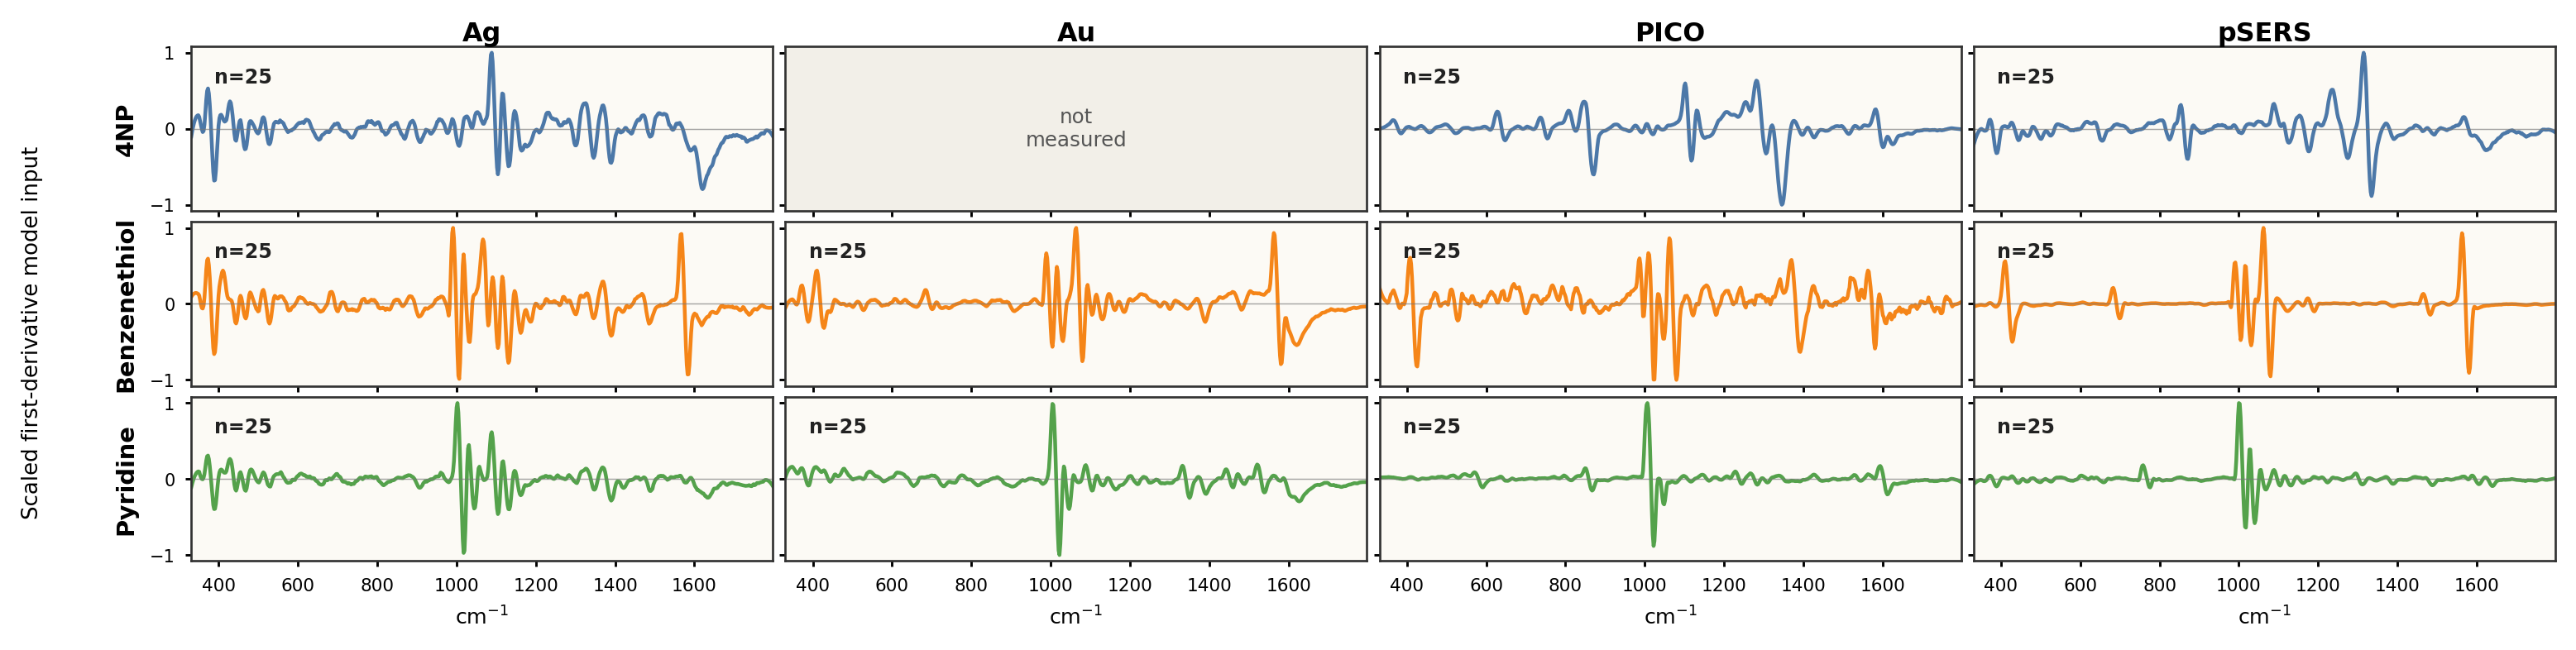
\includegraphics[width=1.22\linewidth]{figures/average_spectra_by_pair_preprocessed_model_compact.png}}
\vspace{-0.06in}
\figcaption{Average first-derivative encoder inputs for the substrate-agnostic model. Spectra are cropped to 330--1800 cm$^{-1}$, SNV normalized, converted to first derivative, and row-L2 scaled before entering the Conv1D encoder.}
\vspace{0.55in}
\tabcaption{Leave-one-substrate-family-out accuracy and macro F1 for each withheld substrate family. Each row tests whether chemical labels learned from the remaining substrate families transfer to the held-out family.}
\tabletext
\begin{tabular}{@{\hspace{0.04in}}lrr@{\hspace{0.04in}}}
\toprule
\textbf{Held out} & \textbf{Acc.} & \textbf{F1} \\
\midrule
Ag & 0.920 & 0.919 \\
Au & 0.980 & 0.990 \\
PICO & 1.000 & 1.000 \\
pSERS & 1.000 & 1.000 \\
\bottomrule
\end{tabular}
\vspace{0.22in}

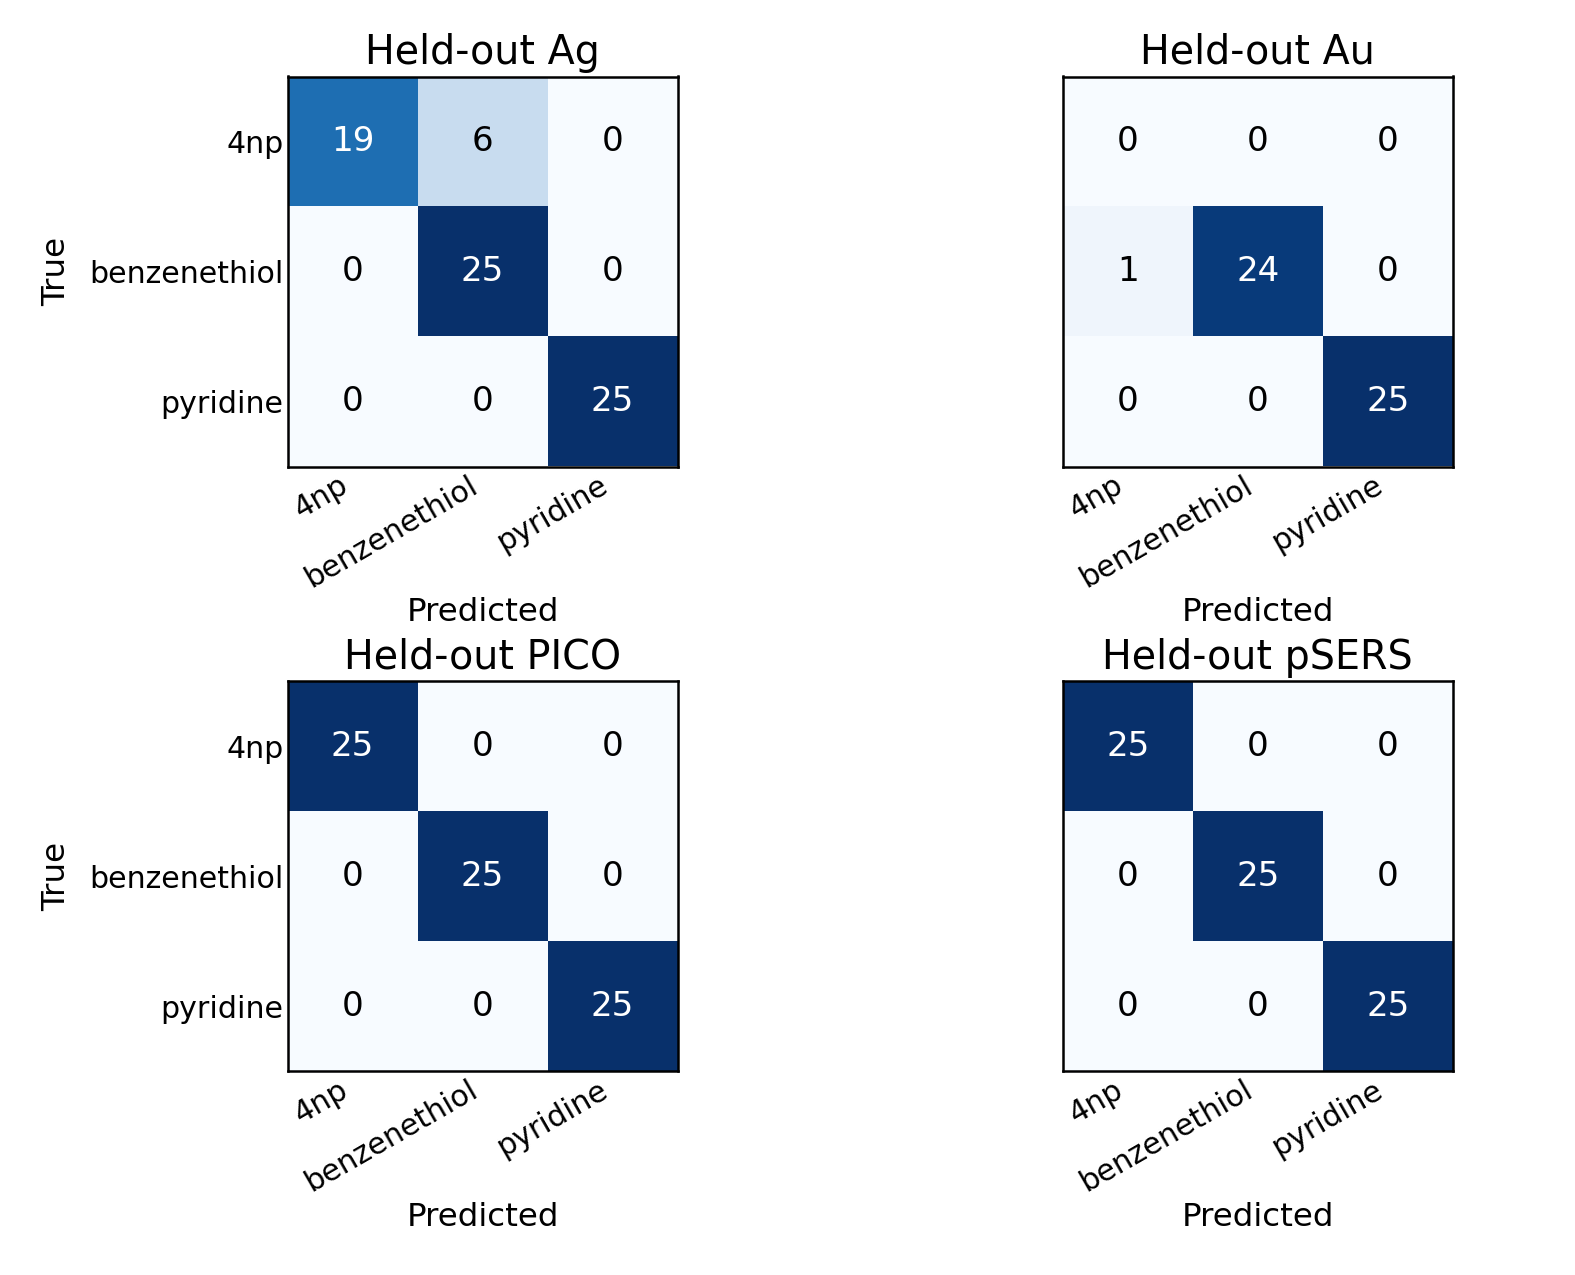
\includegraphics[width=0.94\linewidth]{figures/heldout_confusion_matrices_2x2.png}
\par\begin{center}{\captionfont\color{textblack}\textbf{Figure 9.} Leave-one-substrate-family-out confusion matrices for chemical-label transfer. Each matrix is a true-versus-predicted chemical-label test after excluding one substrate family from training. PICO and pSERS transfer perfectly; Au transfers almost completely but has no 4NP test support because 4NP does not respond on Au. The dominant residual error is held-out Ag, where 6 of 25 4NP spectra are assigned to benzenethiol.\par}\end{center}
\end{minipage}
\hfill
\begin{minipage}[t]{0.50\linewidth}
\vspace{1.00in}
\centering
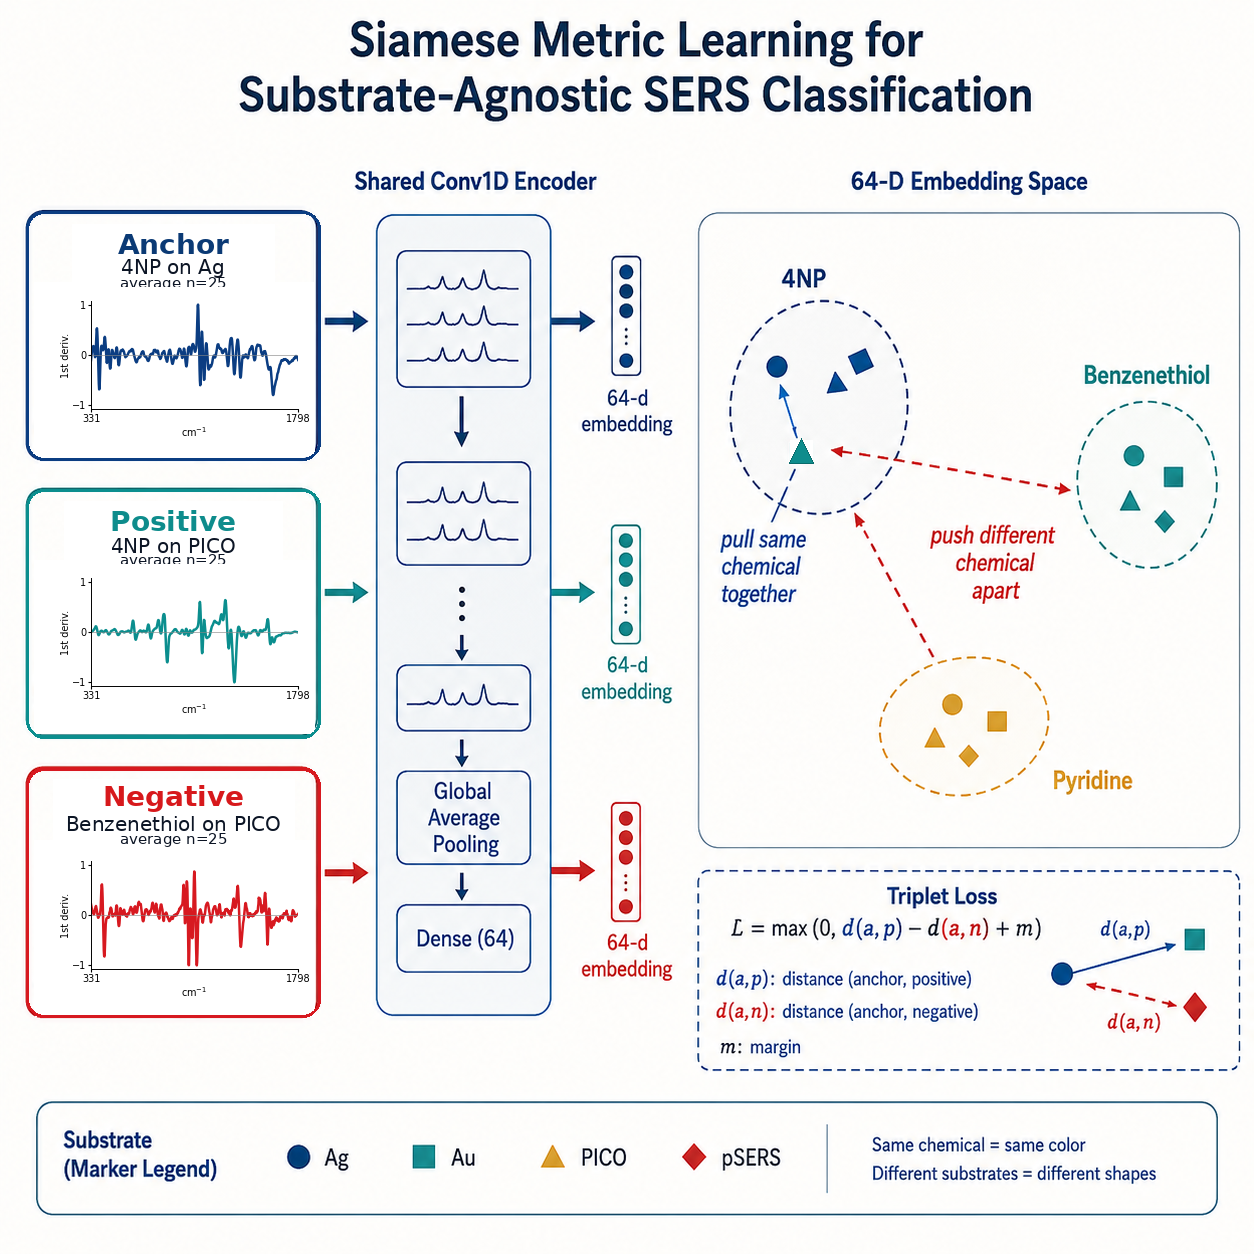
\includegraphics[width=0.64\linewidth]{figures/siamese_metric_learning_4np_pico_positive_average.png}
\figcaption{Triplet-learning schematic for the substrate-agnostic Siamese encoder. The spectra shown at left are averaged encoder inputs after the same preprocessing used for training: crop, SNV normalization, first derivative, and row-L2 normalization. The anchor and positive examples share chemical identity across different substrate families and are pulled together in the learned 64-D embedding space; the negative example is a different chemical and is pushed farther away by the triplet-loss margin. This changes the learned representation from pair identity toward chemical identity across substrates.}
\vspace{0.50in}
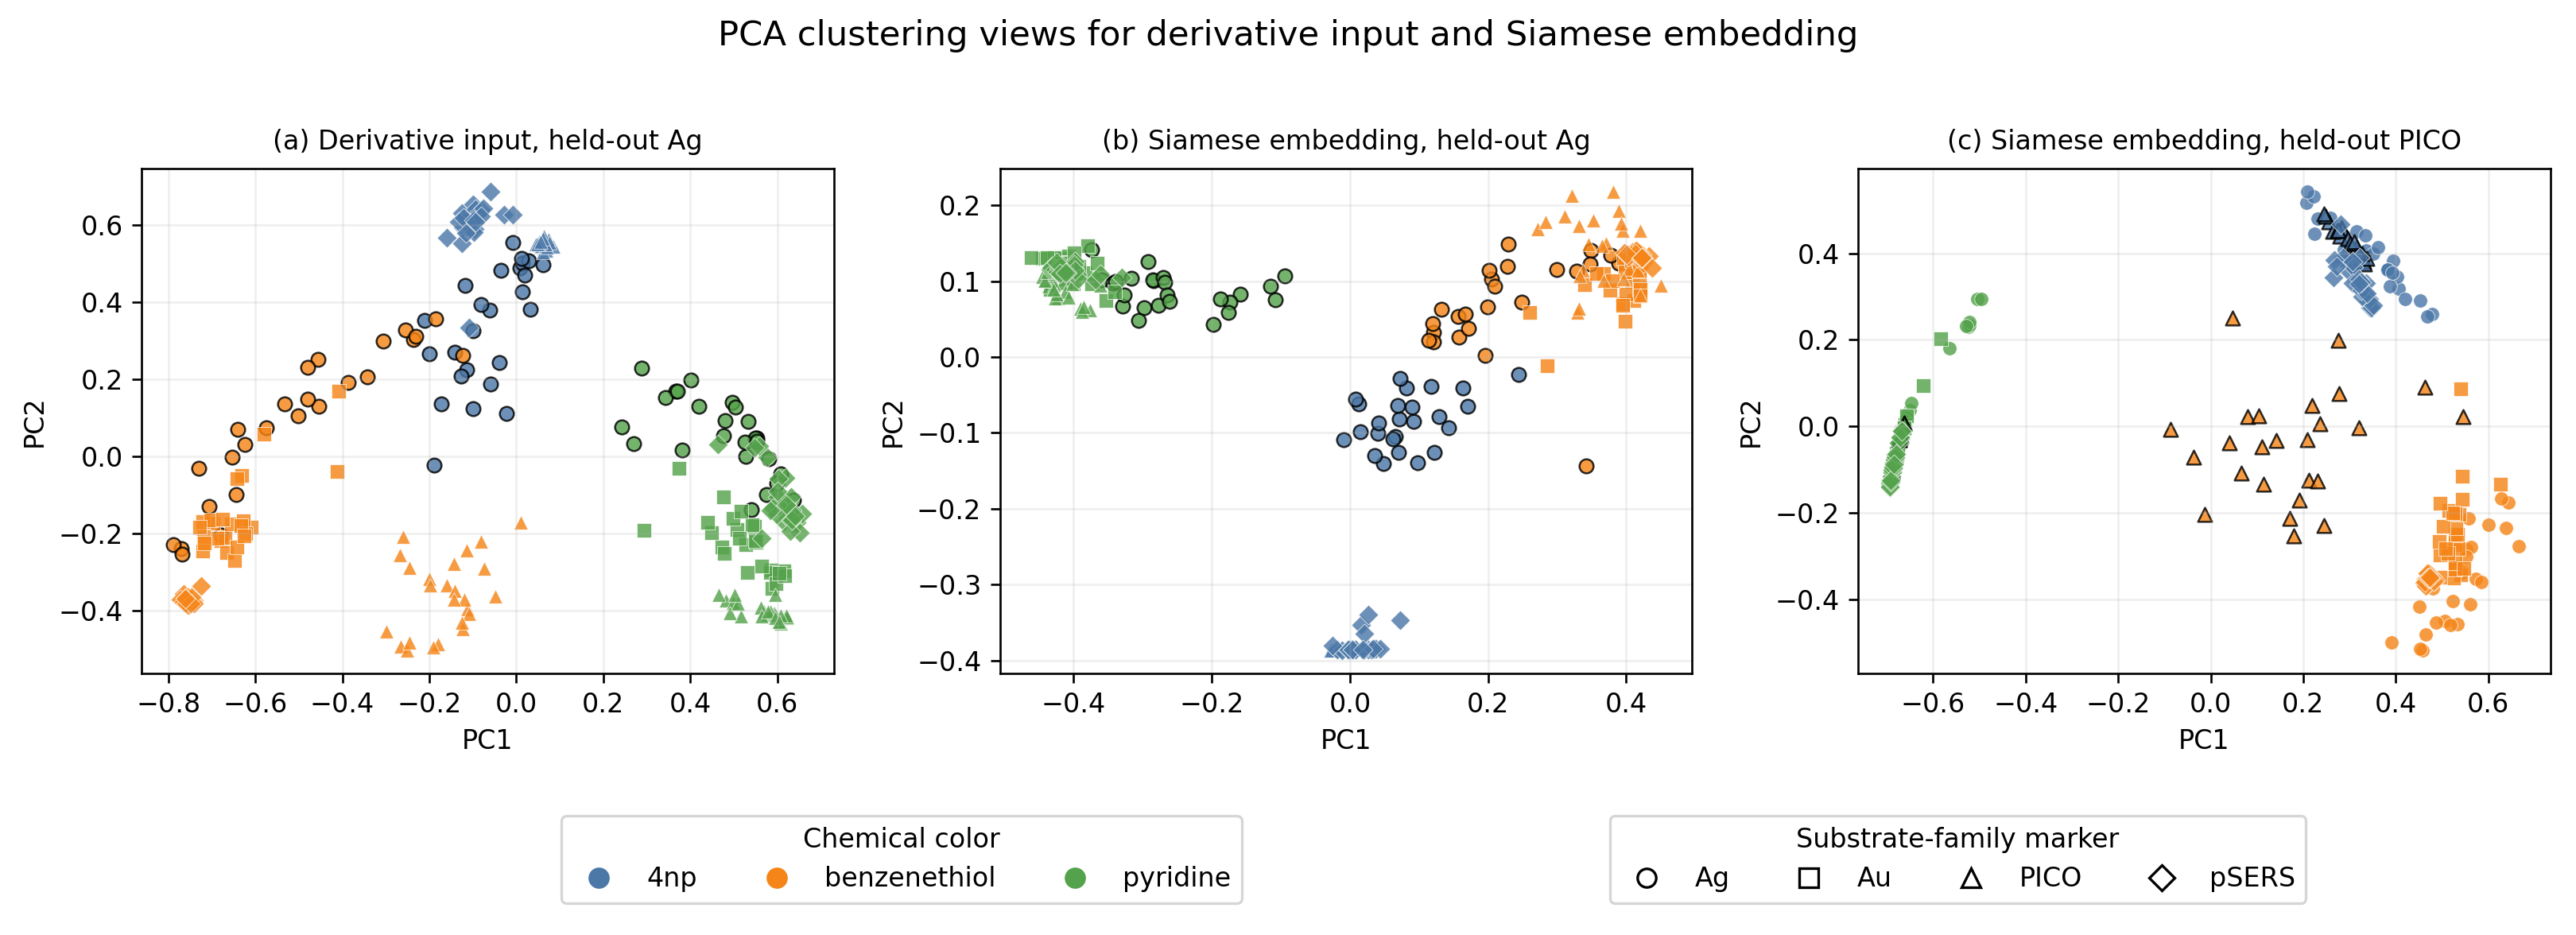
\includegraphics[width=0.98\linewidth]{../sers_substrate_agnostic_supervisor_report/figures/combined_pca_clustering.png}
\figcaption{Compact PCA diagnostic for the substrate-agnostic representation. The derivative-input view shows chemical and substrate effects before metric learning; the embedding views show that the Siamese encoder tightens same-chemical structure while the remaining Ag/4NP weakness appears as a localized overlap.}
\vspace{0.60in}
{\fontsize{16}{19}\selectfont\bfseries\color{templateblue}Geometry shift}\par
{\fontsize{20}{23}\selectfont\bfseries\color{templateaccent}0.837}\hspace{0.04in}{\captionfont label-minus-substrate silhouette gain.}\par
\vspace{0.03in}
\tabcaption{Silhouette comparison for the substrate-agnostic representation. A larger chemical-minus-substrate difference means spectra are organized more by analyte identity than by substrate family.}
\begingroup
\tabletext
\setlength{\tabcolsep}{4pt}
\renewcommand{\arraystretch}{1.02}
\begin{tabular}{@{}lrrr@{}}
\toprule
\textbf{Rep.} & \textbf{Chem.} & \textbf{Sub.} & \textbf{Diff.} \\
\midrule
Input & 0.304 & 0.101 & 0.203 \\
Embedding & 0.797 & -0.040 & 0.837 \\
\bottomrule
\end{tabular}
\endgroup
\end{minipage}

}
\end{minipage}

\end{document}
